% Created by tikzDevice version 0.12.6 on 2026-05-14 20:42:35
% !TEX encoding = UTF-8 Unicode
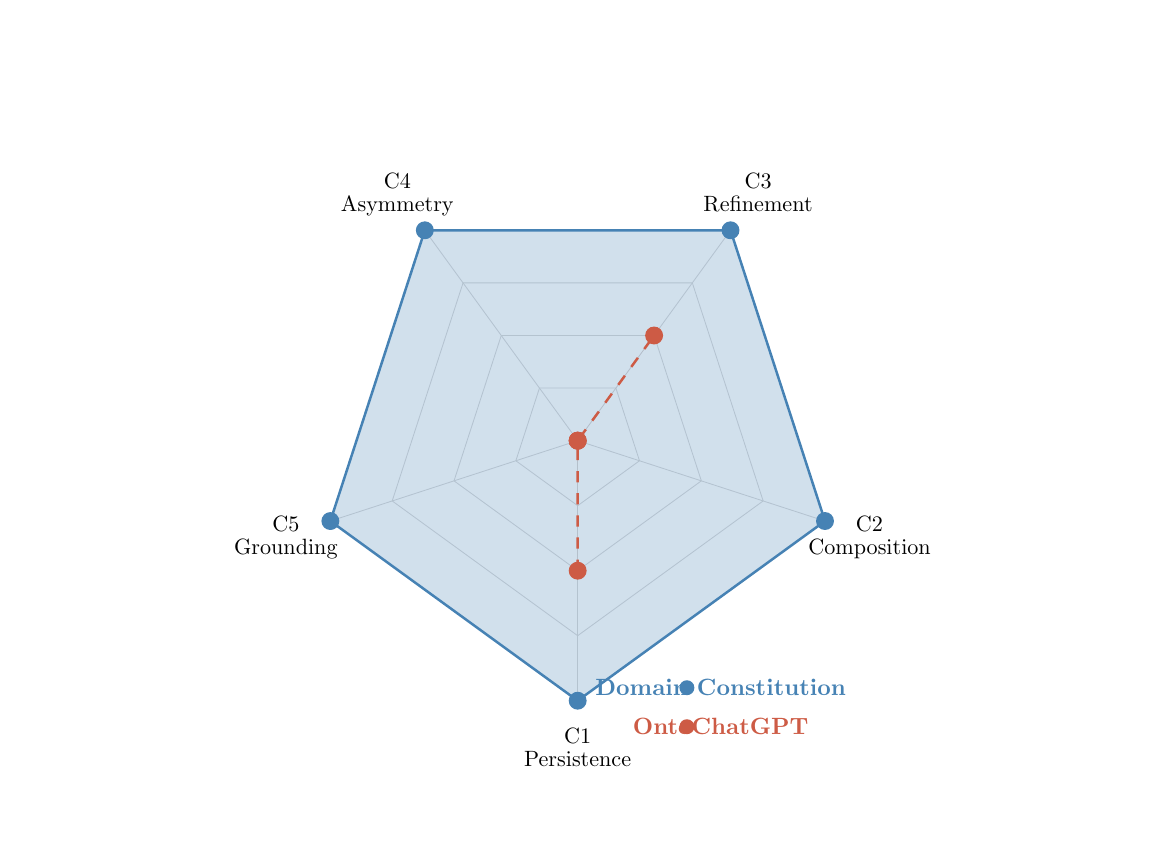
\begin{tikzpicture}[x=1pt,y=1pt]
\definecolor{fillColor}{RGB}{255,255,255}
\path[use as bounding box,fill=fillColor,fill opacity=0.00] (0,0) rectangle (397.48,289.08);
\begin{scope}
\path[clip] ( 49.03,  0.00) rectangle (348.45,289.08);

\path[] ( 49.03,  0.00) rectangle (348.45,289.08);
\end{scope}
\begin{scope}
\path[clip] ( 54.03,  5.00) rectangle (343.45,284.08);
\definecolor{drawColor}{gray}{0.85}

\path[draw=drawColor,line width= 0.3pt,line join=round] (198.74,116.35) --
	(221.08,132.58) --
	(212.55,158.85) --
	(184.93,158.85) --
	(176.40,132.58) --
	(198.74,116.35);

\path[draw=drawColor,line width= 0.3pt,line join=round] (198.74, 92.86) --
	(243.43,125.32) --
	(226.36,177.85) --
	(171.13,177.85) --
	(154.06,125.32) --
	(198.74, 92.86);

\path[draw=drawColor,line width= 0.3pt,line join=round] (198.74, 69.37) --
	(265.77,118.06) --
	(240.17,196.86) --
	(157.32,196.86) --
	(131.72,118.06) --
	(198.74, 69.37);

\path[draw=drawColor,line width= 0.3pt,line join=round] (198.74, 45.88) --
	(288.11,110.80) --
	(253.97,215.86) --
	(143.51,215.86) --
	(109.38,110.80) --
	(198.74, 45.88);

\path[draw=drawColor,line width= 0.3pt,line join=round] (198.74,139.84) -- (198.74, 45.88);

\path[draw=drawColor,line width= 0.3pt,line join=round] (198.74,139.84) -- (288.11,110.80);

\path[draw=drawColor,line width= 0.3pt,line join=round] (198.74,139.84) -- (253.97,215.86);

\path[draw=drawColor,line width= 0.3pt,line join=round] (198.74,139.84) -- (143.51,215.86);

\path[draw=drawColor,line width= 0.3pt,line join=round] (198.74,139.84) -- (109.38,110.80);
\definecolor{drawColor}{RGB}{70,130,180}
\definecolor{fillColor}{RGB}{70,130,180}

\path[draw=drawColor,line width= 0.9pt,line join=round,fill=fillColor,fill opacity=0.25] (198.74, 45.88) --
	(288.11,110.80) --
	(253.97,215.86) --
	(143.51,215.86) --
	(109.38,110.80) --
	(198.74, 45.88) --
	cycle;
\definecolor{drawColor}{RGB}{205,91,69}
\definecolor{fillColor}{RGB}{205,91,69}

\path[draw=drawColor,line width= 0.9pt,dash pattern=on 4pt off 4pt ,line join=round,fill=fillColor,fill opacity=0.20] (198.74, 92.86) --
	(198.74,139.84) --
	(226.36,177.85) --
	(198.74,139.84) --
	(198.74,139.84) --
	(198.74, 92.86) --
	cycle;
\definecolor{drawColor}{RGB}{70,130,180}
\definecolor{fillColor}{RGB}{70,130,180}

\path[draw=drawColor,line width= 0.4pt,line join=round,line cap=round,fill=fillColor] (198.74, 45.88) circle (  3.03);

\path[draw=drawColor,line width= 0.4pt,line join=round,line cap=round,fill=fillColor] (288.11,110.80) circle (  3.03);

\path[draw=drawColor,line width= 0.4pt,line join=round,line cap=round,fill=fillColor] (253.97,215.86) circle (  3.03);

\path[draw=drawColor,line width= 0.4pt,line join=round,line cap=round,fill=fillColor] (143.51,215.86) circle (  3.03);

\path[draw=drawColor,line width= 0.4pt,line join=round,line cap=round,fill=fillColor] (109.38,110.80) circle (  3.03);
\definecolor{drawColor}{RGB}{205,91,69}
\definecolor{fillColor}{RGB}{205,91,69}

\path[draw=drawColor,line width= 0.4pt,line join=round,line cap=round,fill=fillColor] (198.74, 92.86) circle (  3.03);

\path[draw=drawColor,line width= 0.4pt,line join=round,line cap=round,fill=fillColor] (198.74,139.84) circle (  3.03);

\path[draw=drawColor,line width= 0.4pt,line join=round,line cap=round,fill=fillColor] (226.36,177.85) circle (  3.03);

\path[draw=drawColor,line width= 0.4pt,line join=round,line cap=round,fill=fillColor] (198.74,139.84) circle (  3.03);

\path[draw=drawColor,line width= 0.4pt,line join=round,line cap=round,fill=fillColor] (198.74,139.84) circle (  3.03);
\definecolor{drawColor}{RGB}{0,0,0}

\node[text=drawColor,anchor=base,inner sep=0pt, outer sep=0pt, scale=  0.80] at (198.74, 30.28) {C1};

\node[text=drawColor,anchor=base,inner sep=0pt, outer sep=0pt, scale=  0.80] at (198.74, 22.15) {Persistence};

\node[text=drawColor,anchor=base,inner sep=0pt, outer sep=0pt, scale=  0.80] at (304.20,106.90) {C2};

\node[text=drawColor,anchor=base,inner sep=0pt, outer sep=0pt, scale=  0.80] at (304.20, 98.77) {Composition};

\node[text=drawColor,anchor=base,inner sep=0pt, outer sep=0pt, scale=  0.80] at (263.92,230.87) {C3};

\node[text=drawColor,anchor=base,inner sep=0pt, outer sep=0pt, scale=  0.80] at (263.92,222.74) {Refinement};

\node[text=drawColor,anchor=base,inner sep=0pt, outer sep=0pt, scale=  0.80] at (133.57,230.87) {C4};

\node[text=drawColor,anchor=base,inner sep=0pt, outer sep=0pt, scale=  0.80] at (133.57,222.74) {Asymmetry};

\node[text=drawColor,anchor=base,inner sep=0pt, outer sep=0pt, scale=  0.80] at ( 93.29,106.90) {C5};

\node[text=drawColor,anchor=base,inner sep=0pt, outer sep=0pt, scale=  0.80] at ( 93.29, 98.77) {Grounding};
\definecolor{drawColor}{RGB}{70,130,180}

\node[text=drawColor,anchor=base,inner sep=0pt, outer sep=0pt, scale=  0.85] at (250.42, 47.63) {\bfseries Domain Constitution};
\definecolor{drawColor}{RGB}{205,91,69}

\node[text=drawColor,anchor=base,inner sep=0pt, outer sep=0pt, scale=  0.85] at (250.42, 33.53) {\bfseries OntoChatGPT};
\definecolor{drawColor}{RGB}{70,130,180}
\definecolor{fillColor}{RGB}{70,130,180}

\path[draw=drawColor,line width= 0.4pt,line join=round,line cap=round,fill=fillColor] (238.21, 50.57) circle (  2.50);
\definecolor{drawColor}{RGB}{205,91,69}
\definecolor{fillColor}{RGB}{205,91,69}

\path[draw=drawColor,line width= 0.4pt,line join=round,line cap=round,fill=fillColor] (238.21, 36.48) circle (  2.50);
\end{scope}
\end{tikzpicture}
